%
% $RCSfile: framework_example.tex,v $
%
% Copyright (C) 2002-2008. Christian Heller.
%
% Permission is granted to copy, distribute and/or modify this document
% under the terms of the GNU Free Documentation License, Version 1.1 or
% any later version published by the Free Software Foundation; with no
% Invariant Sections, with no Front-Cover Texts and with no Back-Cover
% Texts. A copy of the license is included in the section entitled
% "GNU Free Documentation License".
%
% http://www.cybop.net
% - Cybernetics Oriented Programming -
%
% http://www.resmedicinae.org
% - Information in Medicine -
%
% Version: $Revision: 1.1 $ $Date: 2008-08-19 20:41:06 $ $Author: christian $
% Authors: Christian Heller <christian.heller@tuxtax.de>
%

\subsection{Framework Example}
\label{framework_example_heading}
\index{Framework Example}
\index{Reference Information Model}
\index{RIM}
\index{Health Level Seven}
\index{HL7}
\index{Single Model Approach}
\index{Object Oriented Programming}
\index{OOP}
\index{Top Level Container}
\index{Access Method Elimination}
\index{Knowledge Specification}
\index{Encapsulation}

A much more complex example than the EHR structure demonstrated in section
\ref{association_elimination_heading} is the \emph{Reference Information Model}
(RIM) framework of the \emph{Health Level Seven} (HL7) standardisation
organisation (chapter \ref{res_medicinae_heading}). It is a quite typical
software model, developed in a \emph{Single Model Approach} (section
\ref{single_model_heading}), as it may similarly exist in other business areas.
The coloured legend in figure \ref{rim_figure} helps distinguish the various
parts of the RIM. The part to be picked out to have a closer look here is the
several kinds of RIM \emph{Entities} (figure \ref{entity_figure}).

Diving yet deeper into the framework, one will find the \emph{Person} class,
being a sub class of \emph{Living Subject} (figure \ref{person_figure}). Since
the RIM is an \emph{Object Oriented} (OO) framework, each class will probably
have access methods for all of its attributes. For the \emph{Person} class, the
access methods for \emph{birthdate} and \emph{address} are shown in the figure.
The right-hand side also shows the typical one-line contents of the \emph{set}/
\emph{get} methods, although more code may be put into them, for reasons of
notification, update or others more.

\begin{figure}[ht]
    \begin{center}
        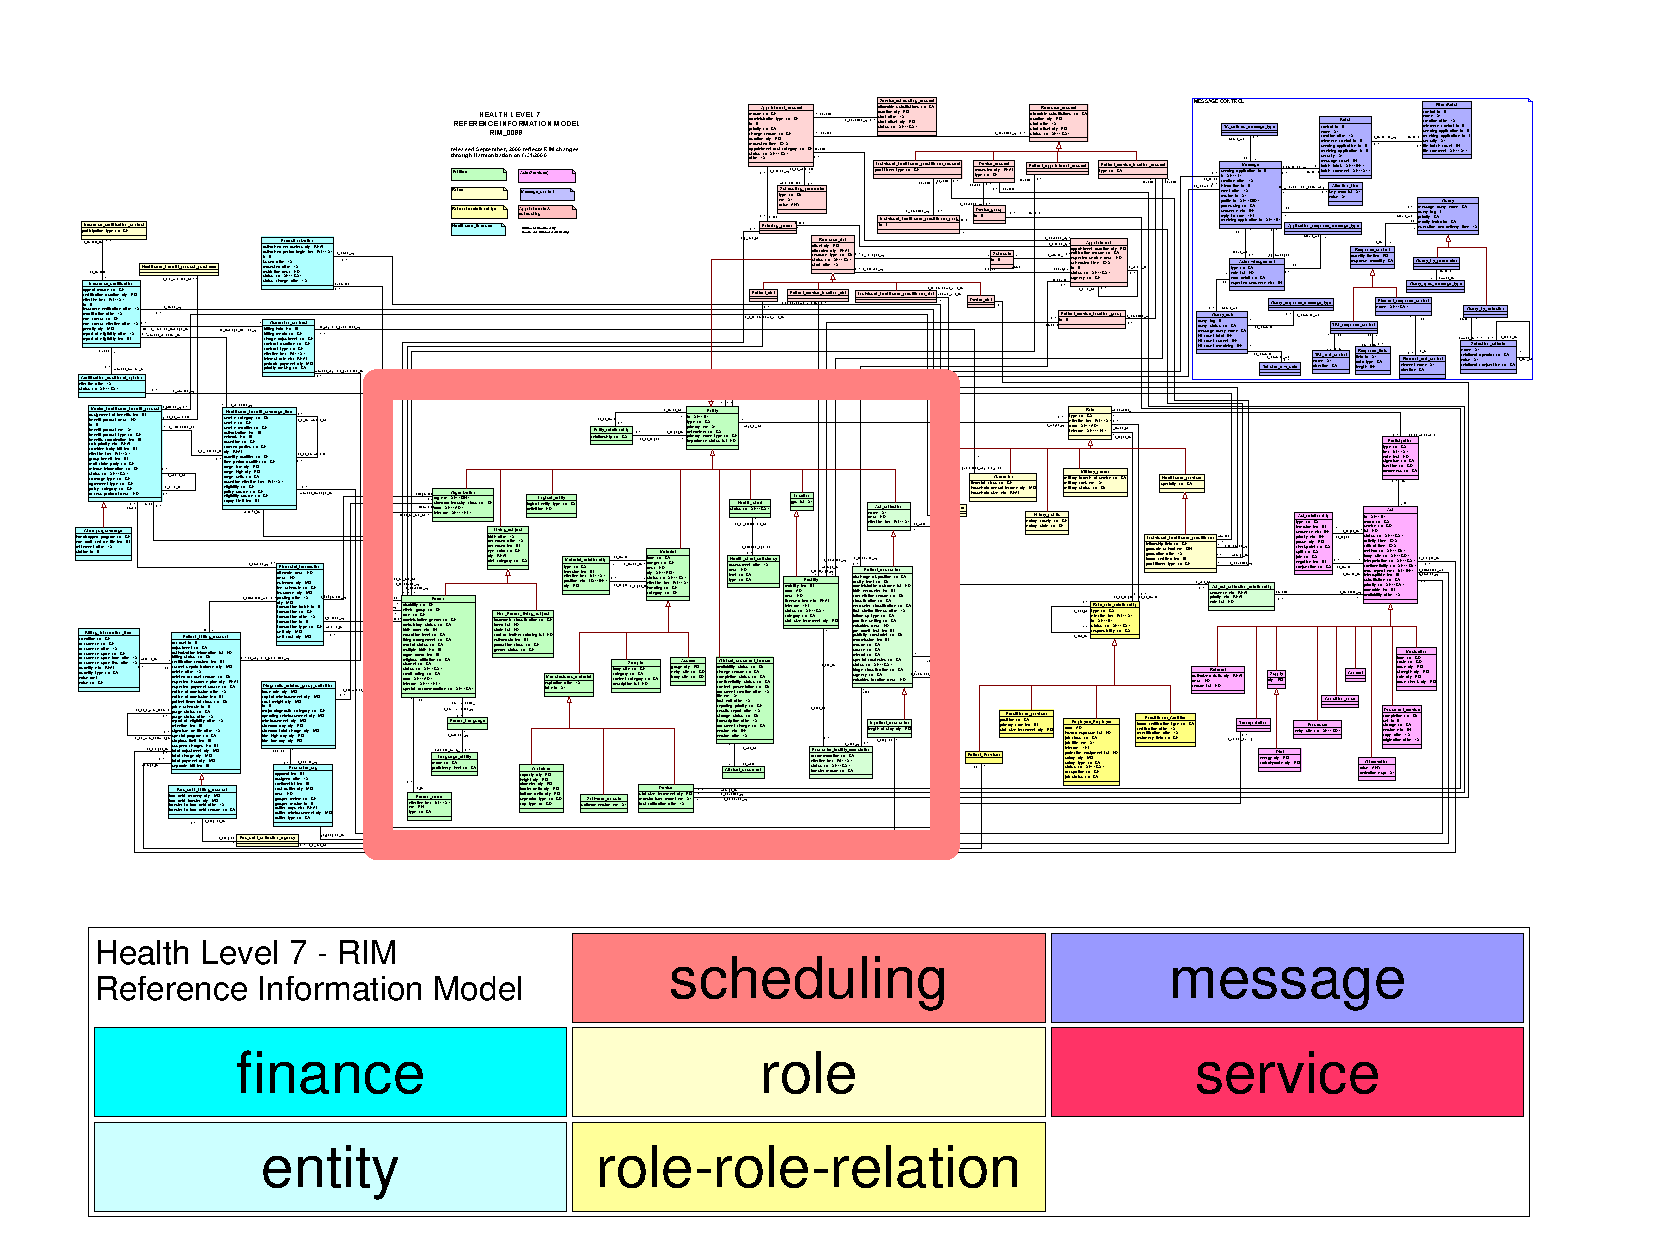
\includegraphics[scale=0.3,angle=-90]{graphic/rim.pdf}
        \caption{HL7 Reference Information Model Framework \cite{hl7}}
        \label{rim_figure}
    \end{center}
\end{figure}

\begin{figure}[ht]
    \begin{center}
        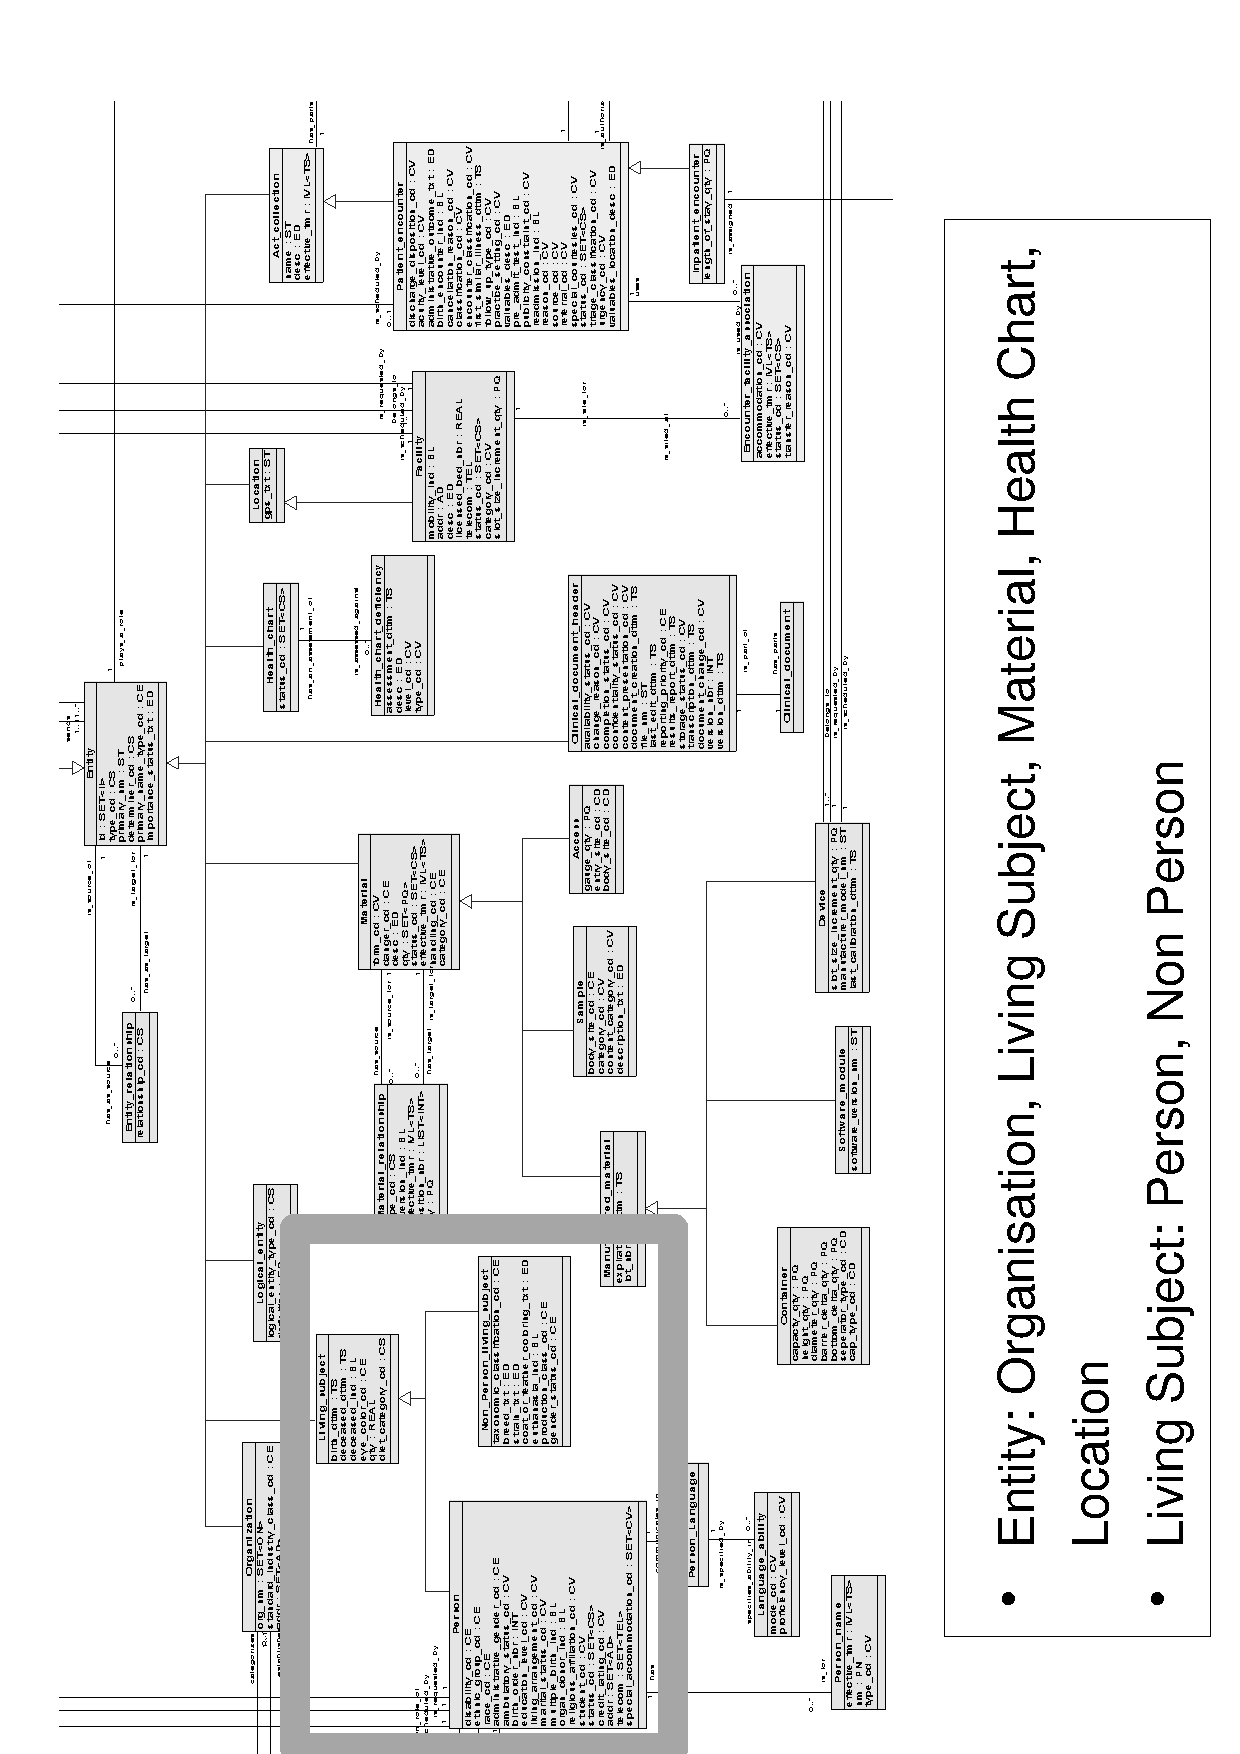
\includegraphics[scale=0.3,angle=-90]{graphic/entity.pdf}
        \caption{RIM Entities \cite{hl7}}
        \label{entity_figure}
    \end{center}
\end{figure}

\clearpage

If the RIM got implemented in the Java programming language, all of its classes
would inherit from the top-most super class \emph{java.lang.Object}. For reasons
of clearity, figure \ref{person_figure} omits several intermediary classes and
lets \emph{Living Subject} inherit directly from \emph{java.lang.Object}.

\begin{figure}[ht]
    \begin{center}
        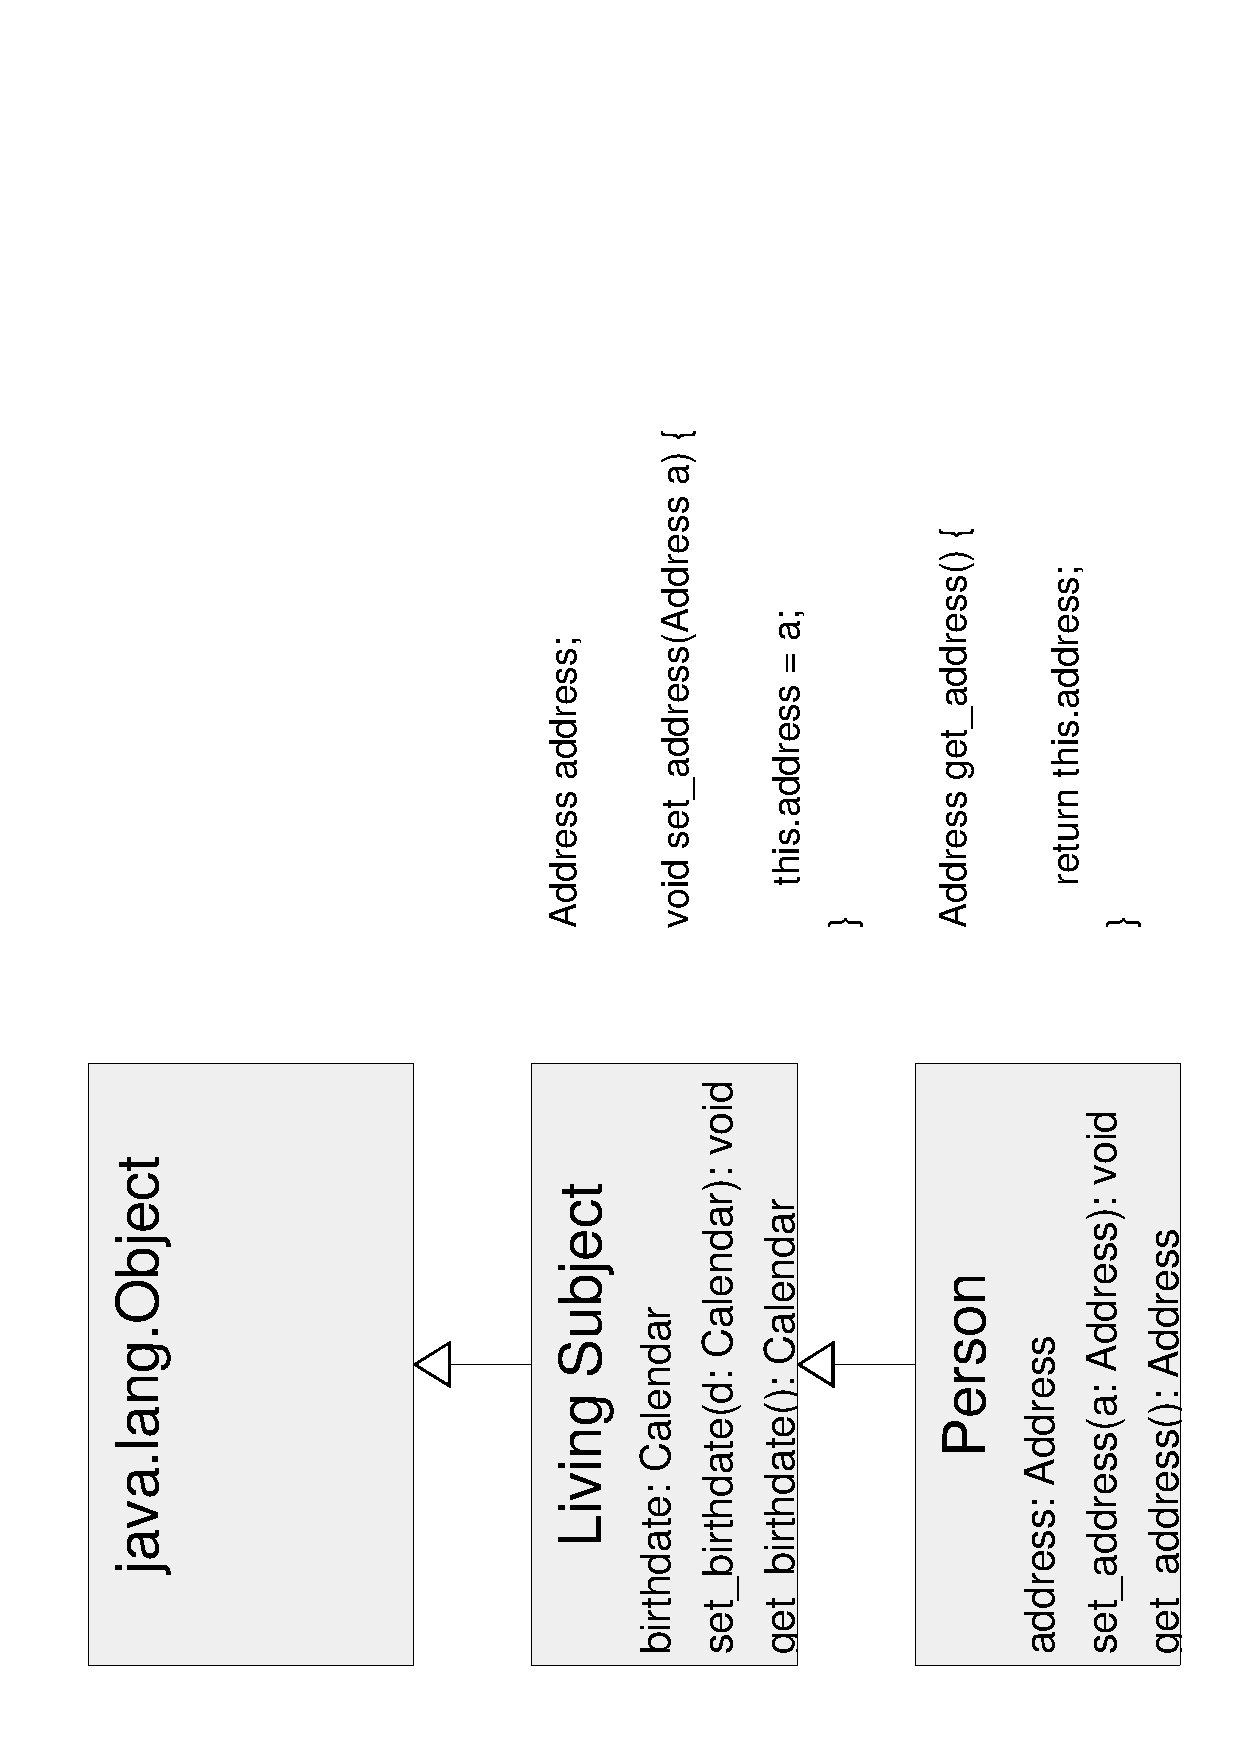
\includegraphics[scale=0.3,angle=-90]{graphic/person.pdf}
        \caption{Accessing a Person's Attributes}
        \label{person_figure}
    \end{center}
\end{figure}

Section \ref{association_elimination_heading} proposed to make the top-most
model in a tree of models inheriting from each other a \emph{Container}. In the
case of Java that would mean to add a container attribute such as one of type
\emph{HashMap}, together with the necessary access methods \emph{set},
\emph{get} and \emph{remove}, to the \emph{java.lang.Object} class (figure
\ref{hashmap_figure}).

That way, every abstract model (OO class) would, by default, become a container
able to store a hierarchy of sub models (objects). This would be much closer to
what section \ref{human_thinking_heading} worked out on the importance of the
principle of \emph{Composition} in human thinking, which perceives its
environment in form of discrete, but composed items. Every item in universe can
be seen as \emph{Compound} of yet smaller items. The basis of every modelling
effort must therefore be a \emph{Container Structure}.

This would also be a solution to the criticism of chapter
\ref{extended_motivation_heading}, meaning that: \textit{the hierarchy as
concept is not inherent in the type system of current programming languages}.

Additionally, access methods of classes inheriting from \emph{java.lang.Object}
(that is of \emph{all} classes) would become superfluous. Because every class
is a sub model of \emph{java.lang.Object}, every class can use not only its
container, but also the corresponding \emph{set}, \emph{get}, \emph{remove}
methods.

\begin{figure}[ht]
    \begin{center}
        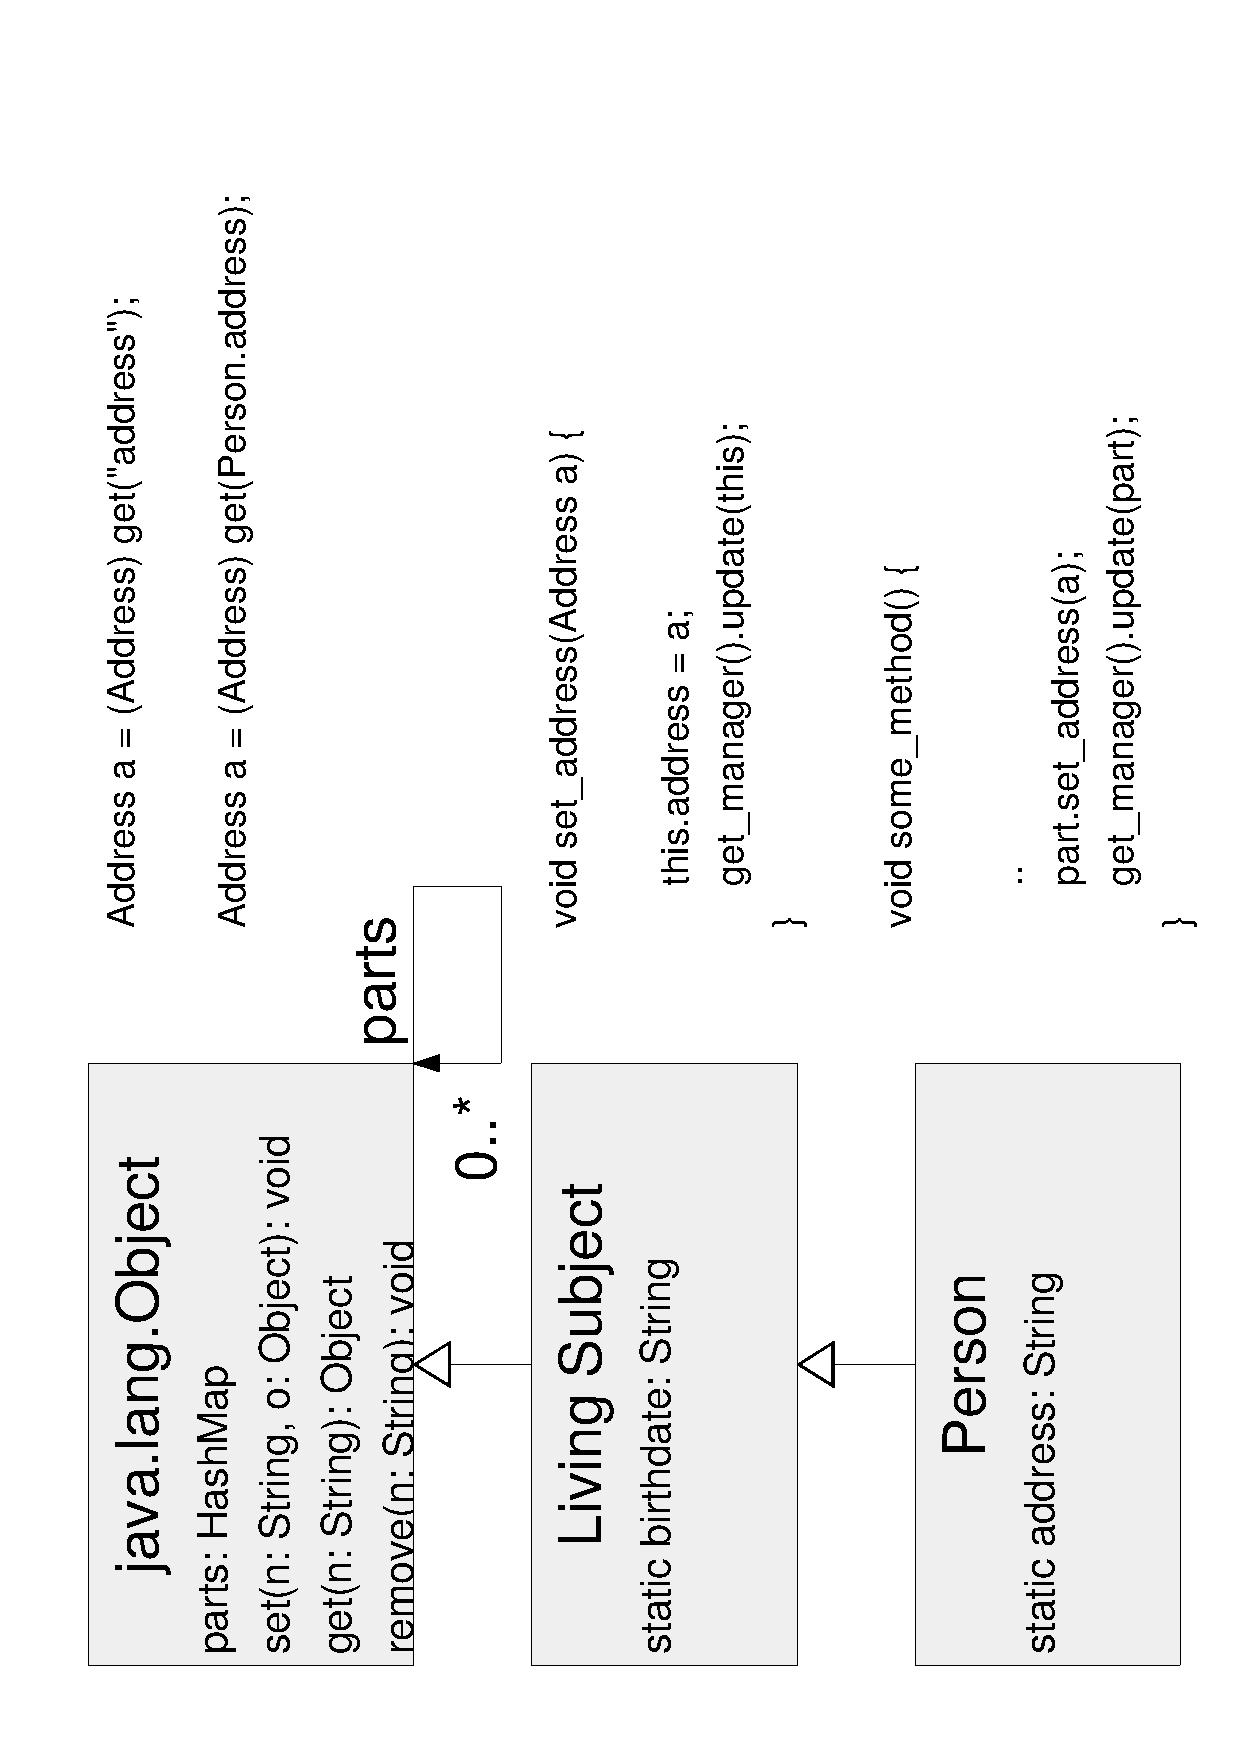
\includegraphics[scale=0.3,angle=-90]{graphic/hashmap.pdf}
        \caption{Access Method Elimination through Top-Level Container}
        \label{hashmap_figure}
    \end{center}
\end{figure}

On its top right-hand corner, figure \ref{hashmap_figure} shows the program code
that could be used to access an \emph{Address} as a \emph{Person}'s sub model.
In order to correctly identify the various attributes of a person, each of them
needs to carry a unique name. In the example of figure \ref{hashmap_figure},
the names are hold as static attributes of the classes they conceptually belong
to. But they can as well be stored somewhere else -- even in an external
configuration file, better called \emph{Knowledge Specification}.

One objection to the elimination of access methods in sub models could be that
then, necessary updates cannot be initiated. Traditionally, such updates are
often placed in the access methods directly. Figure \ref{hashmap_figure} shows
how an update manager is called in the \emph{set\_address} method, after the
\emph{address} attribute has been changed. However, the same update call can be
made outside the access method. It would possibly have to be called at several
places then, but judging from this work's author's experience with frameworks,
the number of update calls won't be too high and is usually well manageable.
The questionableness of the OO principle of \emph{Encapsulation} in general was
already mentioned in section \ref{encapsulation_heading}. Finally, there is
actually no access method-related code that cannot be handled alternatively.
